
\documentclass[english]{article}
\usepackage{graphicx,wrapfig,lipsum}
\usepackage{grffile}
\usepackage{babel}
\usepackage{parskip}
\textwidth = 426pt
\oddsidemargin = 17pt


\title{Coding standards document\\}
\date{\today}


\begin{document}
	\maketitle
	\begin{figure}[!t]
		
\includegraphics{images/up_logo.png}
	\end{figure}
	\begin{minipage}{0.4\textwidth}
		\begin{flushleft} \large
			\textbf{NAMES:}\\[0.4cm]
			Xolo K Dandashe\\
			Phuti K Setoaba\\
			Khodani M Mufamadi
			
		\end{flushleft}
	\end{minipage}
	\begin{minipage}{0.4\textwidth}
		\begin{flushright} \large
			\textbf{STUDENT NUMBER:} \\[0.4cm]
			14245681\\ 	
			13032616\\	
			14197520
		\end{flushright}
	\end{minipage}
	
	
	
	\pagenumbering{gobble}
	\newpage


	\section{Style,Structure and layout}
			
	
		\subsection{Variables, Methods and attributes:}
		\begin{wrapfigure}{r}{5.5cm}
			\caption{Expected representation for naming variables.}\label{wrap-fig:1}
			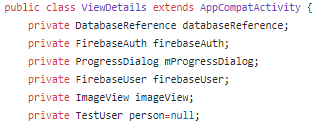
\includegraphics[width=5.5cm]{images/variables.png}
		\end{wrapfigure} 
			$\bullet$\ Should be short and descriptive.\par
			$\bullet$\ Should begin with lower-case letter.\par
$\bullet$\ Upper-case letter should be used immediately after the first name description of the variable.\par
$\bullet$\ Should use a single upper-case letter at the start of each new word within the name.\par
$\bullet$\ Should not be a single character e.g. string x  \par


                                	

		\subsection{Accessor and Mutators}
$\bullet$\  Should have names based on the attribute to which they provide access.\par
$\bullet$\ Should begin with the prefix “get” or “set” followed by the name of the attribute beginning with a capital letter e.g. getItem \par
				
		\subsection{Indentation and Layout}
		$\bullet$\ Blocks that are nested more should be indented more. \par
		
$\bullet$\ Lines should be kept to a sensible length to make the code easier to read and print.\par	
\begin{wrapfigure}{r}{5.5cm}
	\caption{Indentations and Bracketing.}
	\label{wrap-fig:2}
	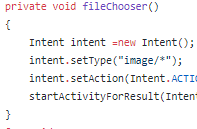
\includegraphics[width=5.5cm]{images/indentation.png}
\end{wrapfigure} 
	$\bullet$\ Single blank lines should be used to separate methods and to emphasise blocks of code.\par	
		
				\subsection{Bracketing}
$\bullet$\ Brackets will be used to clearly show the blocks of code they encapsulate.\par
$\bullet$\ Closing curly brackets should be placed on the line after the last line of the code they enclose, at the same level of indentation as the start of the header on which the block begins. \par
$\bullet$\ Curly brackets should always be used for if-, while- and for-, even when not strictly needed – such as when the body only contains a single statement.\par
\newpage
\subsection{Exceptions}
\begin{wrapfigure}{r}{5.5cm}
	\caption{Exception handling feedback.}
	\label{wrap-fig:3}
	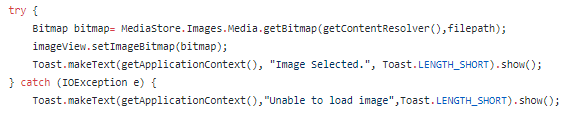
\includegraphics[width=5.5cm]{images/exception.png}
\end{wrapfigure} 
$\bullet$\ Exceptions should be used where necessary.\par
$\bullet$\ Instead of throwing basic Exception classes, sub-classes should be made with more meaningful names.\par
$\bullet$\ Appropriate “catch” statements should be put in place to allow the program to recover if need be.\par




\subsection{Imports}
\begin{wrapfigure}{r}{5.5cm}
	\caption{Expected import use.}
	\label{wrap-fig:4}
	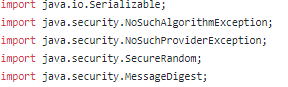
\includegraphics[width=5.5cm]{images/imports.png}
\end{wrapfigure} 
$\bullet$\ Should avoid using import *(importing every package), rather each class should be specifically imported as required.\par

$\bullet$\ Any unused imports should be removed if they are no longer needed to make it clear which classes will be used.\par


				
			\section{Naming Conventions	}
			This section will cover examples referring to some of the conventional rules mentioned above.
				
					\subsection{ Classes }
$\bullet$\ Class names should begin with a capital letter and each new word within the name should begin with a capital letter e.g "ClassName".\par

				\subsection{Exception Classes}
$\bullet$\ Exception classes should follow the same rule as normal classes, but should end with the word Exception e.g "ClassNameException ".\par
\subsection{Methods}
$\bullet$\ Methods should begin with a lower case letter and each new word within the name should begin with a capital letter e.g "methodName()".\par
\subsection{Variables and Attributes }
$\bullet$\ Both variables and attributes should being with a lower case letter and each new word within the name should begin with a capital letter – exactly the same as methods e.g "variableName".\par
\subsection{Packages}
$\bullet$\ Package names should all be in lower case e.g "demo.package".\par

	\section{XML	}
	
	\subsection{Tags}
$\bullet$\ XML tags should be ordered as follows: "xmlns" first, then id,then  \texttt{layout\_width} and  \texttt{layout\_height} alphabetically. \par
$\bullet$\ Add a space between the closing slash and the final attribute.\par E.g.  \texttt{android:textSize="10dp" /> }\par
$\bullet$\ Self closing tags should be used when an XML element doesn't have any contents, you should use self closing tags. \par

\subsection{Layout XML ID Naming / Java Class Widget Declaration Variable}
				
This section provides a guide on how to link xml elements with java variables.
				\\
				\begin{tabular}{ |p{3cm}|p{9cm}|  }
				\hline
				\textbf{Element} & \textbf{Example}  \\
				\hline
				TextView &	TextView textView\\
				\hline
				ImageView &	ImageView imageView\\
				\hline
				Button &	Button button\\
				\hline
				EditText &	EditText editText \\
				\hline
				\end{tabular}
\section{Documentation}

\subsection{Comments}
It is expected that the code written should be structured in a way that all members can understand it without comments but here are some guides to placing comments:\\
$\bullet$\ Use in-line commenting to help the next developer who might be editing your code.\par
$\bullet$\ Inline comments should appear on the line above the code you are commenting.\par
$\bullet$\ Comments should be added within the body of a method if they are used within that method.\par

\subsection{Resource Files}
$\bullet$\ Resources file names should be written in  \texttt{lowercase\_underscore}  e.g  \texttt{ic\_star.png} \par


\subsection{Layout Files}
\begin{wrapfigure}{r}{5.5cm}
	\caption{Layout files.}
	\label{wrap-fig:5}
	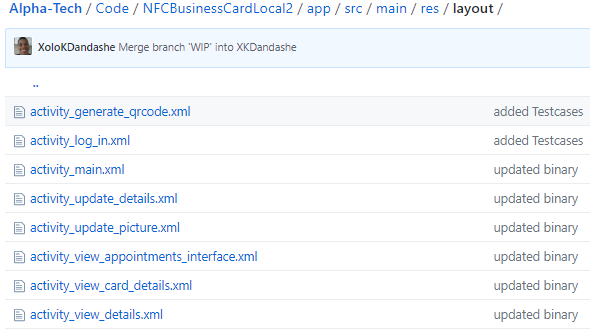
\includegraphics[width=5.5cm]{images/layouts.png}
\end{wrapfigure} 
$\bullet$\ Layout files should match the name of the Android components that they are intended for but moving the top level component name to the beginning. \par
$\bullet$\ Example, if you are creating a layout for the SignInActivity, the name of the layout file should be \texttt{activity\_sign\_in.xml} \par



\subsection{Version control}
$\bullet$\ No commented out code must be committed unless you have a very good reason that is clearly described in a comment by the code you are committing. \par


\subsection{Repository definitions}
\begin{wrapfigure}{r}{5.5cm}
	\caption{Java files.}
	\label{wrap-fig:6}
	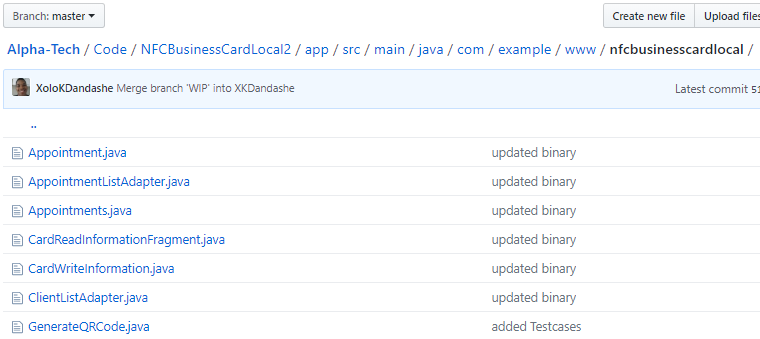
\includegraphics[width=5.5cm]{images/javafiles.png}
\end{wrapfigure} 
$\bullet$\ All the pictures should be in a folder called images. \par
$\bullet$\ All the files should belong to a specific folder. \par
$\bullet$\ Folder names should be descriptive enough to show what they contain. \par

\section{Code quality}
$\bullet$\ We need to ensure that we keep at least a 70\% overall correspondence with the coding standards guidelines to ensure that we have a high level of code quality.\par

$\bullet$\ These guidelines are for us to follow as much as possible to ensure production time is minimized and that we do not waste resources trying to explain each other when integration is needed.\par
$\bullet$\ A high level of code quality will enable us to produce better components, improve testing and minimize confusion. \par 
$\bullet$\ Reviews will be simpler to perform and improvements will be simpler to implement.\par

$\bullet$\ Android Studio will be used for development which uses Java for backend functions and XML for layout presentation. \par
$\bullet$\ Coding standard rules mentioned above will be used for resources naming conventions, formatting and also to ensure version control.
 \par
 $\bullet$\ Commit frequently to ensure no important information is lost.
 \par

\section{Repository}
\begin{wrapfigure}{r}{5.5cm}
	\caption{Branching Structure.}
	\label{wrap-fig:7}
	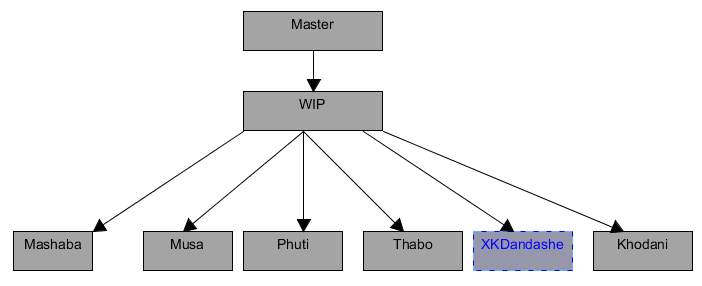
\includegraphics[width=5.5cm]{images/Branching.png}
\end{wrapfigure}
Our Github repository is Alpha-Tech. We use the team name so that members can identify the repository easier in the case of a member having multiple repositories that they are working on. 
\subsection{Branching and Merging}		
Our repository has a tree like logic-representation where each member is expected to have a branch of their own, a work-in-progress (WIP) branch and the master at the top:\\
$\bullet$\ The structure of how the work will be presented is created in the master branch.\par
$\bullet$\ Once we have set up the master branch, a work-in-progress (WIP) branch is created then clones the master to have the same file structure and layout.\par 
\begin{wrapfigure}{r}{5.5cm}
	\caption{Merging branches.}
	\label{wrap-fig:8}
	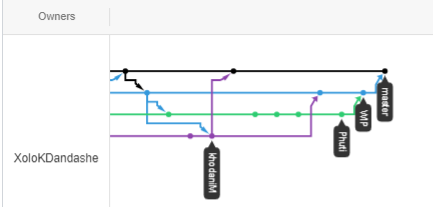
\includegraphics[width=5.5cm]{images/merging.png}
\end{wrapfigure}
$\bullet$\ The WIP branch is the hub where all members can pull and push their work that has not been reviewed but has been completed.\par
$\bullet$\ Once the work completed, in WIP, is reviewed by other members, then it is pushed to the master.\par
$\bullet$\ No member may commit directly into the master branch or are allowed to push and/or pull from the master due to how it contains ready to be deployed work.\par 
$\bullet$\ A member may merge their branch with WIP only once they have completed all the work they have been assigned.\par
$\bullet$\ If a member has merged their branch with WIP then they may delete their branch as for the work will be in the WIP branch which will be later merged with master once all the work is reviewed. \par


\end{document}
